% -*- coding: utf-8 -*-
% !TEX encoding = UTF-8 Unicode
% !TEX root =  main.tex

\chapter{Grundlagen der Vektorregelung}
\label{cha:Grundlagen der Vektorregelung}

%% -- Einführung in die Vektorregelung
In modernen Antriebssystemen ist es häufig unerlässlich, entscheidende Maschinengrößen wie Drehzahl oder Drehmoment auf einen gewünschten Wert einzustellen.
Dabei kamen der Vergangenheit häufig Gleichstrommaschinen zum Einsatz, welche sich durch eine gute Regel- und Einstelleigenschaften bei den geforderten Parametern auszeichnen.
Große Fortschritte in den Bereichen der Leistungselektronik und bei Regelkomponenten führen dazu, dass heute Antriebe, ohne besonderen Aufwand, mit Synchronmaschinen realisiert werden können.
Gleichzeitig haben die Drehfeldmaschinen den Vorteil, dass Aufgrund der fehlenden mechanischen Kommutation kein nennenswerter Verschleiß Auftritt.

Entscheidend für den Aufbau einer geregelten PMSM ist die Vektor- bzw.\ feldorientierte Regelung. 
Die Maschine wird mit näherungsweise sinusförmig veränderlichen Strömen gespeist. 
Ebenso besitzen alle weiteren auftretenden elektrischen Größen wie Spannungen, Flüsse oder Felder aufgrund ihres Zeitverhaltens annähernd Sinusform \parencite[S.~1]{nuss2010}.	
Die Idee der Vektorregelung ist es nun, nicht die zeitlichen Momentanwerte der Ströme zu verändern, sondern die erfassten Wechselgrößen in ein Zwei-komponentiges rotierendes Koordinatensystem zu übertragen.
Diese Komponenten werden regelungstechnisch verwertet und zurück transformiert.

\section{Raumzeigerdarstellung}
\label{sec:raumzeiger}

Die stationären Zusammenhänge der elektrischen Größen in der Maschine, welche ursächlich aus dem Zusammenhang von $\Psi$ und B herrühren, können zunächst mithilfe komplexer Zeitzeiger beschrieben werden. Dabei lassen sich die Statorströme, $i_{s,1}$, $i_{s,2}$, und $i_{s,3}$ einer Drehfeldmaschine mit idendischer Amplitunde $\hat i_{s}$ und Statorkreisfrequenz $\omega_{s}$  und einer jeweiligen $120^\circ$ Phasenverschiebung als

\begin{align}
	\begin{split}
	i_{s,i} = Re\{\underline{i}_{s,i}\} = Re\{\underline{\hat i}_{s,i}\cdot e^{j\omega_{s}t}\} = Re\Bigl\{\hat{i_{s}}\cdot e^{j(\omega_{s}t+0-(i-1)\cdot\tfrac{2\pi}{3})}\Bigr\}
	\\= \hat{i}_{s}\cdot cos\bigg(\omega_{s}t+\varphi_{0}-(i-1)\cdot\frac{2\pi}{3}\bigg)~;~mit~i=1,2,3 \label{statorströme} 
\end{split}
\end{align}

mit den komplexen Zeitzeigern

\begin{align}
	\underline{i}_{s,i} = \underline{\hat i}_{s,i}\cdot e^{j\omega_{s}t}~;~mit~i=1,2,3 \label{zeitzeiger}
\end{align}

und den komplexen Amplituden

\begin{align}
	\underline{\hat i}_{s,i} = \hat{i_{s}}\cdot e^{j(\omega_{s}t+0-(i-1)\cdot\tfrac{2\pi}{3})}~;~mit~i=1,2,3 \label{amplituden}
\end{align}

darstellen. 
Die folgende Abbildung \ref{fig:zeitzeiger} veranschaulicht die vorangegangenen Gleichungen \ref{statorströme}, \ref{zeitzeiger} sowie \ref{amplituden} und stellt beispielhaft den Zeitzeiger $i_{s,1}$ dar.

\begin{figure}[h]
	\centering
	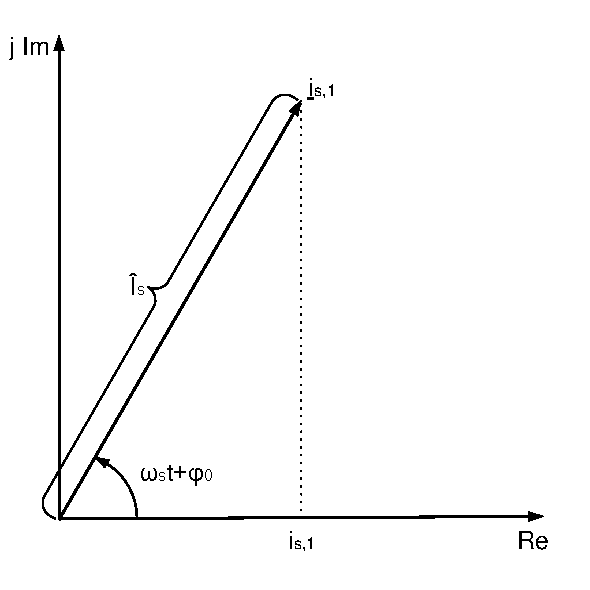
\includegraphics[width=0.5\textwidth]{zeitzeiger.pdf}
	\label{fig:zeitzeiger}
	\caption{Beispielhafte Lage eines Zeitzeigers.}
\end{figure}

Da das Ziel darin besteht, den dynamischen Rotationsvorgang einer PMSM zu modellieren, ist die Verwendung eines Zeitzeigers, mit dem nur stationöre Vorgänge beschrieben werden können, nicht angebracht. 
Hier ist es Zweckmäßig, einen Operator so zu entwickeln, dass dieser in der Lage ist, dynamische Vorgänge zu beschrieben, ohne dazu Nebenbedingungen wie beispielsweise die Periodizität heranzuziehen. 
Bei der Entwicklung bieten sich die Statorphasenströme $i_{s,1}$, $i_{s,2}$, und $i_{s,3}$ des Dreiphasensystems an.
Diese stehen zu jedem Zeitpunkt zur Verfügung. 
Es sei angemerkt, dass dabei die Nullbedingung erfüllt ist. 
Die Summe der Statorphasenströme muss immer null sein, was beim Einsatz von Drehfeldmaschinen idr. gegeben ist.
Dadrurch ist es auch immer möglich mit Kenntnis zweier Größen auf die dritte zu schließen.
Nun ist zweikomponentige Zeitzeiger immer um mindestens zwei Momentanwerte erweiterbar. 
Ein hierfür geeigneter Ansatz zur Erzeugung eines Raumzeigers wurde erstmals in kovacs1959 veröffentlicht:

\begin{align}
	\underline{i}_{s}(t) = \frac{2}{3} \cdot \Bigl\{\underline{i}_{s,1}(t) + \underline{i}_{s,2}(t)\cdot e^{j\tfrac{2\pi}{3}} + \underline{i}_{s,3}(t)\cdot e^{j\tfrac{4\pi}{3}} \Bigr\} \label{statorstromzeiger}
\end{align}

Um jetz aufzeigen zu können, dass der Ansatz aus \ref{statorstromzeiger} im stationären Zustand mit dem entsprechenden Statorstromzeitzeiger übereinstimmt und schlussendlich den Raumzeiger zu erzeugen, werden zunächst in \ref{statorstromzeiger} die Statortrommomentanwerte aus \ref{statorströme} eingesetzt.
Dadurch erhält man

\begin{align}
\underline{i}_{s}(t) = \frac{2}{3} \cdot \biggl\{\hat{i}_{s}\cdot cos(\omega_{s}t+\varphi_{0}) + \hat{i}_{s}\cdot cos\bigg(\omega_{s}t+\varphi_{0}-\frac{2\pi}{3}\bigg)\cdot e^{j\tfrac{2\pi}{3}} + \hat{i}_{s}\cdot cos\bigg(\omega_{s}t+\varphi_{0}-\frac{4\pi}{3}\bigg)\cdot e^{j\tfrac{4\pi}{3}} \biggr\}
\label{zwischen1}
\end{align}

Wird nun die trigonometrische Cosinus-Funktion durch die entsprechende exponentielle Darstellung ersetzt, folgt hieraus

\begin{align}
	\begin{split}
	\underline{i}_{s}(t) = \frac{2}{3} \cdot \hat{i}_{s} \cdot \biggl\{ \frac{1}{2} \cdot ( e^{j(\omega_{s}t+\varphi_{0})} + e^{-j(\omega_{s}t+\varphi_{0})} ) + \frac{1}{2} \cdot ( e^{j(\omega_{s}t+\varphi_{0}-\frac{2\pi}{3})} + e^{-j(\omega_{s}t+\varphi_{0}-\frac{2\pi}{3})})\cdot e^{j\tfrac{2\pi}{3}} + \\ \frac{1}{2} \cdot ( e^{j(\omega_{s}t+\varphi_{0}-\frac{4\pi}{3})} + e^{-j(\omega_{s}t+\varphi_{0}-\frac{4\pi}{3})})\cdot e^{j\tfrac{4\pi}{3}}  \biggr\}
	\label{zwischen2}
	\end{split}
\end{align}

Nach ausmultiplizieren der Therme folgt mit $1+e^{j\tfrac{4\pi}{3}}+e^{j\tfrac{8\pi}{3}}=0$ das Ergebnis und somit der Raumzeiger

\begin{align}
	\underline{i}_{s} = \frac{2}{3} \cdot \hat{i}_{s}\cdot\biggl\{ \frac{3}{2} \cdot  e^{j(\omega_{s}t+\varphi_{0})} + \frac{1}{2} \cdot e^{-j(\omega_{s}t+\varphi_{0})} \cdot \bigg( 1+e^{j\tfrac{4\pi}{3}}+e^{j\tfrac{8\pi}{3}} \bigg)  \biggr\} = \hat{i}_{s} \cdot e^{j(\omega_{s}t+\varphi_{0})}
	\label{zeigerende}
\end{align}

Das Ergebnis von \ref{zeigerende} entspricht strukturell dem in \ref{statorströme} angegebenen Statorstromzeitzeiger. Dadurch ist sichergestellt, dass der Ansatz aus \ref{statorstromzeiger} in der Lage ist als Gesamtzeiger, bestehend aus den Momentanwerten der Statorströme, zu fungieren. 
Die folgende Abbildung \ref{fig:raumzeigermaschine} zeigt zur Veranschaulichung eine zweipolige Drehfeldmaschine mit zugehörigem Zeigerdiagramm, welches den Statorstromraumzeiger beinhaltet. 

\begin{figure}[h]
	\centering
	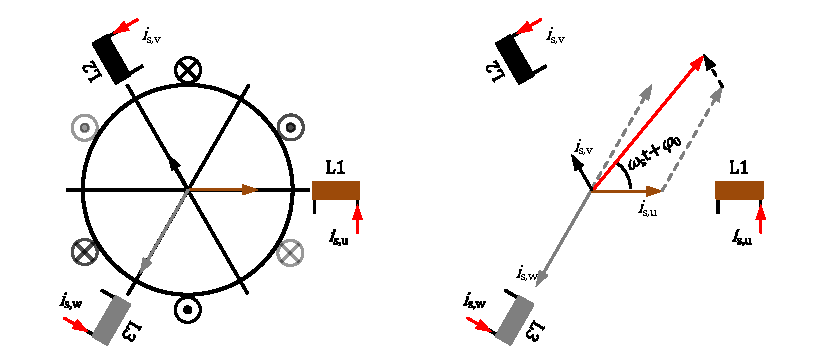
\includegraphics[width=0.5\textwidth]{raumzeigermaschine.pdf}
	\label{fig:raumzeigermaschine}
	\caption{zweipolige Drehfeldmachine mit beispielhafter Statorstromraumzeigerlage}
\end{figure}

Mit der Einführung des Raumzeigers ist die theoretische Grundlage dafür geschaffen, die PMSM mit einer feldorientierten Regelung zu versehen. 
Da sich wie Eingangs beschrieben alls Größen in der Drehfeldmaschine näherungsweise sinusförmig verhalten, ist die Stromraumzeigerdarstellung aus \ref{statorstromzeiger} für alle andren dreiphasigen Größen als allgemeine Raumzeigerdarstellung definierbar.

\begin{align}
	\underline{a}(t) = \frac{2}{3} \cdot \Bigl\{\underline{a}_{1}(t) + \underline{a}_{2}(t)\cdot e^{j\tfrac{2\pi}{3}} + \underline{a}_{3}(t)\cdot e^{j\tfrac{4\pi}{3}} \Bigr\} \label{raumzeigerdefinition}
\end{align}

Im Folgenden werden die in der Praxis benötigten Transformationsvorschriften erläutert, welche das Wechseln zwischen Phasen- und Raumzeigergrößen erlauben.


\section{Beschreibung in $\alpha$-$\beta$-Koordinatensystem}\label{sec:clark}

Als Grundlage für das Wechseln zwischen Phasen- und Raumzeigergrößen dienz zunächst die Definition aus \ref{raumzeigerdefinition}. Die Definitionsgleichung lässt sich in Real- und Imaginärteil aufspalten. Es kommt so zu folgender Aufteilung

\begin{align}
	Re{\underline{a}(t)} =
	\label{realteil}
\end{align}

\begin{align}
	\label{imaginärteil}
\end{align}

\section{Beschreibung in rotorfesten d-q-Koordinatensystem}\label{sec:park}

%\section{Einführung in die Raumzeigermodulation}\label{sec:raumzeiger}

%\subsection{Begriff des Raumzeigers}

\subsection{Transformation zwischen Phasen- und Raumzeigergrößen}

\subsection{Raumzeigertransformation zwischen ortsfesten und rotierenden Bezugssystemen}

\section{Signalflussplan der Vektorregelung}\label{sec:signalflussplan}



%%% Local Variables: 
%%% mode: latex
%%% TeX-master: "main"
%%% TeX-open-quote: "\\enquote{"
%%% TeX-close-quote: "}"
%%% LaTeX-csquotes-open-quote: "\\enquote{"
%%% LaTeX-csquotes-close-quote: "}"
%%% End: 
